%!TEX root = bioPrediction_main.tex

\subsection{Minimum Number of Training Samples}\label{secLearningCurve}
Collecting experience samples from users is expensive, since participants 
are being interrupted several times a day and have to answer the survey. 
To minimize the number of samples to be collected from participants, we 
examined how the performance of individual classifiers changes over the 
number of samples used to train the classifier.

Participants in our study had varying levels of responsiveness to the 
experience sampling ranging from 10 to 76 (see Figure~
\ref{responseDistribution}).
%Answering Reviewer 2's concern: Why only 10 participants? What was the rationale for the cut-off selected? 
To answer this research question we analyze the maximum number of responses \textbf{all} analyzed participants have to train the model. Since some participants have a very small number of maximum answers (ten being the lowest) we excluded the four participants with the least number of responses for this analysis.
%To maintain a certain generalizability while 
%also being able to examine a range of sample numbers for training the 
%classifier, we removed the four participants with the least number of 
%samples for this analysis. 
As a result, we obtained a corpus of analysis where all participants have a 
higher number of responses (34 being the lowest), which allows us to examine 
the learning curve of the classifiers for a larger number of training data points. For our 
analysis, we thus performed a leave-one-out cross validation with random 
sample sets of size 1 to 33 and calculated the average through all folds of 
the validation.

For each of the three productivity-related aspects, we are again more 
interested in predicting when a worker is stressed, not awake, or not 
focused, the less common class in all three cases. Since the less common 
class can be very small, we weighted each participants' classifier 
performance by the percentage of the samples in this smaller class.

\begin{figure}
  \centering
          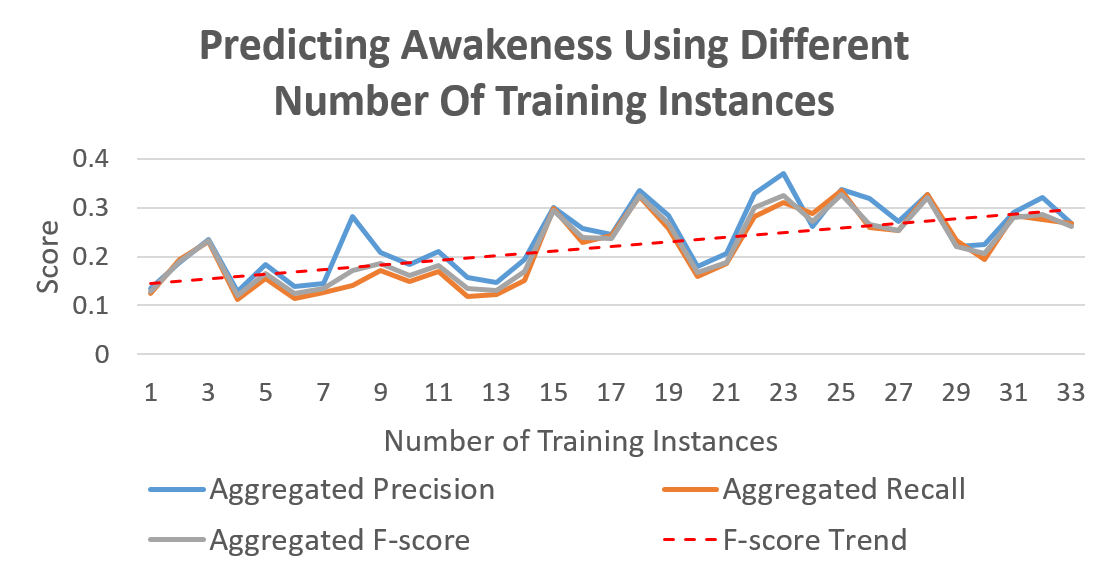
\includegraphics[width=0.5\textwidth]{20180912AwakenessLC2.png}
  \caption{Performance of the per participant trained awakeness classifiers, measured in precision, recall (sensitivity), and F-score. The dotted red line represents the F-score trend.}\label{fig:learningCurveInd}
  %\vspace*{-3mm}
\end{figure}

%\vspace{0.05in}
\noindent\textit{Individual Classifiers for Binary Prediction}\\
The averaged performance of all individually trained random forest classifiers for 'awake' with respect to the training sample size is presented in Figure~\ref{fig:learningCurveInd}. The trend indicates a positive correlation between the number of samples in the training set and the classifiers' F-score performance, with an overall improvement of  114\% (from 0.14 to 0.30) in the F-score between a training set of one sample to one with 33 samples. The trends for
the remaining indicators are 29\% for stress and no overall improvement for focus.%\\[-0.1cm]

%\noindent\textit{}
%When contrasting
%models trained and tested on the 
%biometric data of each user individually, against
%a general model trained and tested with the data of all users. 
%We can conclude
%that for up to 33 training samples analyzed in this study,
%the former has better performance when predicting the
%responses of each user than when training 
%a model with the data of several different users. 
%This is partially due to the 
%variability across users and the subjective nature
%of the responses (e.g.,where slightly awake for one person
%may be not awake for another). 

\begin{figure}
  \centering
      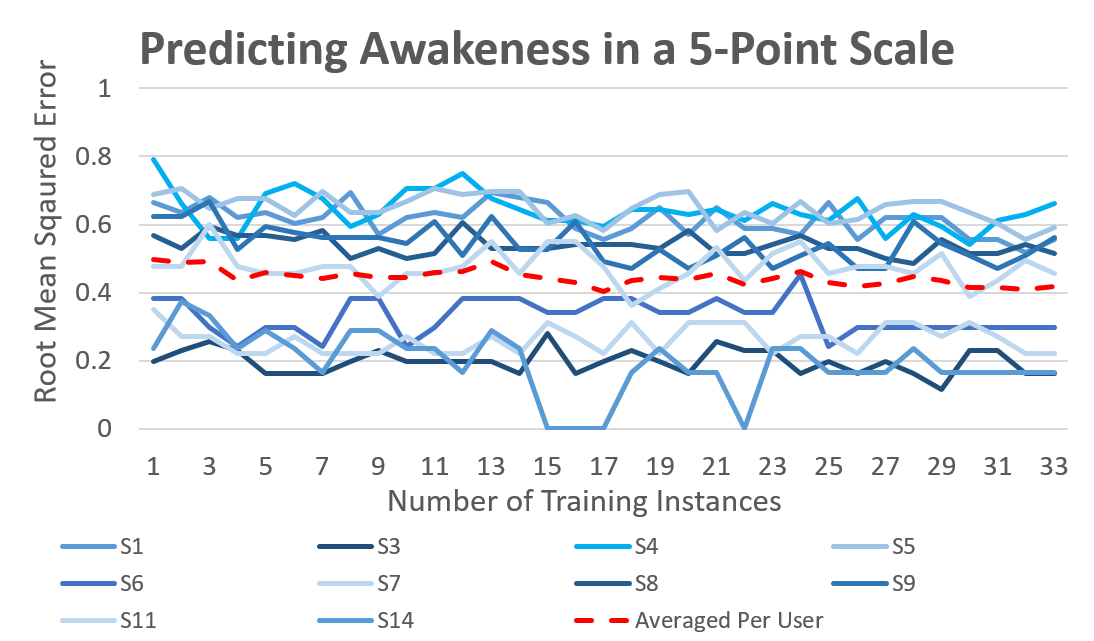
\includegraphics[width=0.5\textwidth]{20180914Awakeness5PointScaleOnly15Lines.png}
  \caption{Performance of the per participant trained classifiers for predicting 5-point awakeness, measured in root mean squared error.}
   \label{fig:learningCurve5}
\end{figure}

\noindent\textit{Predicting Five Classes}\\
In a second step, we analyzed a more fine-grained prediction using the initial 5-point Likert scale responses rather than the binarized ones as output measure. Figure~\ref{fig:learningCurve5} depicts the performance of the individually trained classifiers in terms of the root mean squared error. The root mean squared error represents the distance of the predicted from the actual value, which provides a more nuanced measure of the performance in the fine-grained prediction case. The figure shows a similar trend as for the binarized prediction, in that the root mean square error averaged over all ten participants decreases with more samples (from 0.49 to 0.41 root mean square error) and thus the performance increases. At the same time, the figure also shows that the performance results for the fine-grained prediction, again, vary substantially across participants.

\subsection{Minimum Time Window}\label{secMinimumTW}
In general, the less biometric data is needed to accurately predict a certain outcome measure, the easier and faster the analysis and data collection. To examine the optimal and minimum time window for the prediction of stress, focus, and awakeness, we used 16 different time windows from 10 seconds to 3 hours as depicted in Figure~\ref{timeWindows}. For our analysis, we then trained individual classifiers for each of the 16 time windows, using only features that had a time window smaller or equal to the time window rather than using all combinations of $\{Biometric Measures\} X \{Statistical Metrics\} X \{Time Windows\}$. We again used random forest and a leave-one-out cross validation to train individual classifiers. Since the number of features used for the training changed with each time window, we did not apply our feature selection in this case, but used all features available. Finally, due to the imbalance in the data, we again weighted each participants' classifier performance by the number of instances in the smaller class to calculate the average.

\begin{figure}
  \centering
      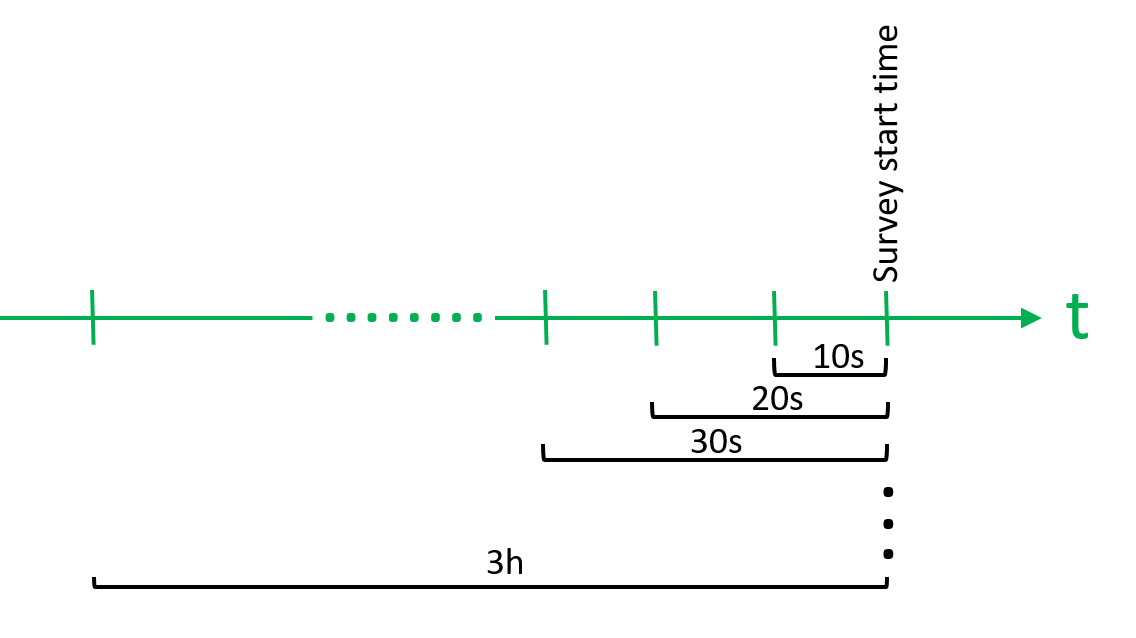
\includegraphics[width=0.4\textwidth]{timeWindows.png}
  \caption{Time windows of biometric data collected prior to each survey response: 10sec, 20sec, 30sec, 45sec, 1min, 2min, 3min, 5min, 7.5min, 10min, 20min, 30min, 45min, 1hour, 2hour, and 3hour.}
   \label{timeWindows}
\end{figure}

Figure~\ref{timeWindowsPandR} shows how the F-score changes for predicting 
`awake' over the 16 different time windows. The figure shows an increasing 
trend in the F-score, i.e. the higher the number of included time windows, 
the higher the F-score. However, there is one exception, the time window of 
1200 seconds that achieves a performance close to the one for the time 
window 10,800 seconds (3 hours), at which point all features are included. 
Overall, our results thus show that while using all time windows up to 3 
hours performs best, and outperforms the feature set that is solely based on 
a 10 second time window by 28\% (from 0.18 to 0.24), the performance for a 
time window of 1200 seconds is a good trade-off for selecting a shorter time 
window while maintaining high performance.

\begin{figure}
  \centering
      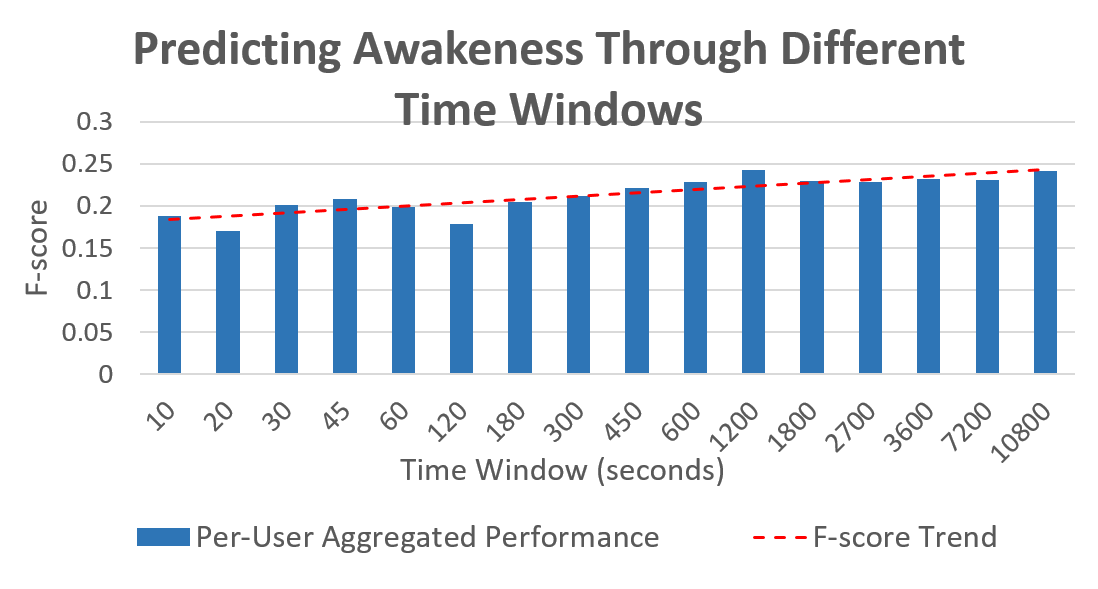
\includegraphics[width=0.5\textwidth]{20180912AwakenessTWBars.png}
  \caption{Performance (F-score) of individual classifiers trained on the different time windows to predict `awake'.}
  \label{timeWindowsPandR}
 % \vspace*{-3mm}
\end{figure}

%We also compared the performance of a model created per user against
%a model created across users.
%To calculate the performance of the model created per user,
%for each user we create a model using the features 
%related to each time window for the selected user only, 
%while in the model created with data across users,
%we trained the model with the data related to each
%particular time window of all users.
%our results show that the personalized model created
%for each user outperforms in every case
%the model created the with data across all users.

%This study
%shows that in general larger time windows predict stress,
%focus, and awakeness more precisely than 
%shorter time windows. We can also notice
%a very gentle upwards trend
%with a inflexion points at 45 seconds and 180.
%There is a peak of performance in 45 seconds, 
%time window that could be used if time is a scarce resource.
%The performance stabilizes around 180 time window
%which indicates that collecting data for a longer time
%period will not increase significantly the performance of the approach.
%The difference in performance between the 
%lowest performing and the highest performing time window is 
%less than a 10\% improvement. 


\subsection{Computer Interaction Data} \label{secCI}
Given our focus on knowledge workers (i.e., workers who generally spend a lot of time interacting with information on their computer at work), we also analyzed the use of computer interaction features to predict focus, awakeness and stress. To collect computer interaction data, we used an open source computer interaction monitor (reference omitted for double-blind.)
%the open source PersonalAnalytics project\footnote{https://github.com/sealuzh/PersonalAnalytics}  \cite{meyer18} 
to track participant's mouse and keyboard activity, as well as details about their active window. The specifics of the features tracked are listed in Table \ref{tracker}. The tracker was installed on the computers of 10 of the 14 participants, with participants S6, S10, S12, and S13 opting out of this part of the study due to privacy concerns.  Therefore, we limited this analysis to the 10 participants for whom we could calculate all features. 

\begin{table}
\begin{center}
\small\addtolength{\tabcolsep}{-1pt}
\begin{tabular}{l l}
\hline

Feature collected by tool & Description \\ 
\hline
Total keystrokes per min& Sum of all types of keystrokes \\ 
Normal keystrokes per min&F[h] Not backspace and navigation \\ 
Backspace keystrokes per min& Backspace keystrokes \\ 
Navigation keystrokes per min& Arrow key keystrokes \\ 
Total clicks per min& Sum of all click types \\ 
Other clicks per min& Not right and left clicks \\ 
Left clicks per min& Left clicks \\ 
Right clicks per min& Right clicks \\ 
Scrolled distance per min& Scrolled distance in pixels \\ 
Moved distance per min& Mouse movements in pixels \\ 
Activity switches per min& Browser window title changes \\ 
Category switches per min& Activity performed category \\ 
\hline
\end{tabular}
\caption{Features collected per user by the computer interaction tracker}%~\cite{meyer18}}
\label{tracker}
\end{center}
%\vspace*{-1mm}
\end{table}

For calculating computer interaction features, we again used the aforementioned 16 time windows and scaled the computer interaction values if the time windows did not align. For our comparative analysis of the different sensing techniques---biometrics vs computer interaction---we then created two new feature sets for each participant in addition to the biometric one: one with only computer interaction features, and one with computer interaction features plus biometric features. 

Table~\ref{ciPerformance} lists the results of our analysis. The results show that in all cases, the computer interaction based model was able to improve upon the biometric model in terms of precision and recall.
%MS is removing the accuracy results because it is not what we care about and it is just making the results harder to understand
%, but not in accuracy. 
Further, we found that the combined model was the most effective model in terms of precision and recall for predicting stress and awakeness overall, but performed slightly worse than the model using only computer interaction features for focus. 
%Since we consider precision and recall for predicting the class of higher interest, i.e. stressed, not focused, not awake, to be the most important statistics when interpreting our results, we compared the models against each other by averaging these two statistics.


\begin{table}
\begin{center}
%\small\addtolength{\tabcolsep}{-1pt}
\begin{tabular}{llllll}
\hline
Model/Feature Set & Precision & Recall & F-Score \\ %& Accuracy\\
\hline
\textbf{Awakeness}\\
\hspace{3mm}Biometrics only  & 0.269 & 0.314 & 0.289 \\ %& 0.808\\
\hspace{3mm}C.I. only  & 0.425 & 0.362 & 0.391 \\ % & 0.758\\
\hspace{3mm}Biometrics + C.I. & 0.390 & 0.404 & 0.400 \\ % & 0.791 \\
\hline
\textbf{Stress}\\
\hspace{3mm}Biometrics only  & 0.270 &	0.260 & 0.265 \\ % & 0.775\\
\hspace{3mm}C.I. only & 0.290 & 0.272 & 0.281 \\ % & 0.698 \\
\hspace{3mm}Biometrics + C.I. & 0.317 & 0.286 & 0.301 \\ % & 0.712\\
\hline
\textbf{Focus}\\
\hspace{3mm}Biometrics only & 0.251 & 0.256 & 0.253 \\ % & 0.716\\
\hspace{3mm}C.I. only & 0.332 & 0.342 & 0.337 \\ % & 0.742\\
\hspace{3mm}Biometrics + C.I. & 0.340 & 0.316 & 0.328 \\ % & 0.745\\
\hline
\end{tabular}
\caption{Comparison of the performance of predicting stress, focus and awakeness using the 3 different feature sets for the 10 participants. The performance is calculated as the average of the performance of the individual classifiers. Computer Interactions is abbreviated as C.I. here for readability. Precision and recall refer to the prediction of the more important classes, i.e. `stressed', `not awake', `not focused'.}
\label{ciPerformance}
\end{center}
%\vspace*{-1mm}
\end{table}

As with the biometric models, the individual performance of both the computer interaction only models and the combined models varied quite a bit between participants. Using stress as an example again, in the computer interaction models 5 of the 10 participants saw improvements compared to the baseline, with a maximum improvement of 128\% in precision, and 78\% in recall. In the combined model for stress, 5 of the 10 participants saw improvements compared to the baseline, with a maximum improvement of 117\% in precision and 95\% in recall. Neither model was capable of correctly predicting any instances of 'stressed' for participant S7.

Since the number of features changes  depending on which feature set is used, we adjusted the feature selection parameter for each of the computer interaction and combined computer interaction/biometric models. The values reported in this section were achieved using the optimal feature selection parameters we found, which are shown in Table \ref{ciFeatureSelection}.

\begin{table}
\begin{center}
\begin{tabular}{lc}
\hline
Model/Feature Set & Number of Features Selected\\
\hline
\textbf{Stress}\\
\hspace{3mm}C.I. & 400\\
\hspace{3mm}Biometrics + C.I. & 800\\
\hline
\textbf{Focus}\\
\hspace{3mm}C.I. & 20\\
\hspace{3mm}Biometrics + C.I. & 300\\
\hline
\textbf{Awakeness}\\
\hspace{3mm}C.I. & All\\
\hspace{3mm}Biometrics + C.I. & 50\\
\hline
\end{tabular}
\caption{The optimal number of features we found to select for each of the model/feature set combinations. Computer interactions is abbreviated as C.I.}
\label{ciFeatureSelection}
\end{center}
\vspace*{-4mm}
\end{table}

